\documentclass[14pt]{article}
\usepackage{listings}
\usepackage{color}
\usepackage{graphicx}
\usepackage{setspace}
\usepackage{mathtools}
\usepackage{amsmath}

\definecolor{dkgreen}{rgb}{0,0.6,0}
\definecolor{gray}{rgb}{0.5,0.5,0.5}
\definecolor{mauve}{rgb}{0.58,0,0.82}

\lstset{frame=tb,
  language=Java,
  aboveskip=3mm,
  belowskip=3mm,
  showstringspaces=false,
  columns=flexible,
  basicstyle={\small\ttfamily},
  numbers=none,
  numberstyle=\tiny\color{gray},
  keywordstyle=\color{blue},
  commentstyle=\color{dkgreen},
  stringstyle=\color{mauve},
  breaklines=true,
  breakatwhitespace=true
  tabsize=3
}

\begin{document}
\title{\huge \textbf{Synchronization Mechanisms Lab Assignment} }
\date{\today}
\maketitle
\begin{center}
\vspace{30 mm}

\title{\huge \textbf{Student: Brinzan Florinel-Razvan}}
\\\vspace{10 mm}
\title{\huge Calculatoare si tehnologia informatiei (limba romana)}
\\\vspace{10 mm}
\title{\huge \textbf{C.R 3.1 A}}
\\\vspace{10 mm}
\title{\huge \textbf{Anul 3}}
\date{}
\maketitle

\newpage
\end{center}

\section{Problema 2 -- Problema cinei filosofilor}

\vspace{4 mm}

\subsection{Enuntul problemei}

\vspace{2 mm}


\textbf{--- Implementați problema cinei filosofilor folosind:}

\begin{enumerate}
\item \textbf{semafoare}
\item \textbf{monitoare }
\item \textbf{lacate}
\end{enumerate}

\begin{center}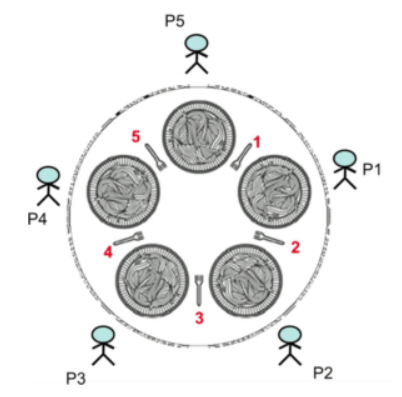
\includegraphics[height=3 in, width = 3 in]{filosofi.png}
\end{center}

\textbf{Pe scurt}, la o masa sunt \textbf{5 filosofi si 5 furculite}. Filosofii fac doua activitati separate: se gandesc si mananca. 

\vspace{2 mm}

\textbf{Pentru a manca, un filosof are nevoie de doua furculite}. Asta inseamna ca pentru a manca toti cei 5 filosofi in acelasi timp ar fi nevoie de 10 furculite ( ceea ce nu este posibil ). 

\vspace{2 mm}

\textbf{Doi filosofi alaturati impart aceeasi furculita.}

\vspace{2 mm}

\textbf{Spre exemplu:}

\vspace{2 mm}

\textbf{Filosofului 1 ii apartine:}
\begin{itemize}
\item \textbf{\textit{furculita 1}}
\item \textbf{\textit{furculita 2}}
\end{itemize}


\textbf{Filosofului 2 ii apartine:}
\begin{itemize}
\item \textbf{\textit{furculita 2}}
\item \textbf{\textit{furculita 3}}
\end{itemize}


\textbf{Filosofului 3 ii apartine:}
\begin{itemize}
\item \textbf{\textit{furculita 3}}
\item \textbf{\textit{furculita 4}}
\end{itemize}


\textbf{Filosofului 4 ii apartine:}
\begin{itemize}
\item \textbf{\textit{furculita 4}}
\item \textbf{\textit{furculita 5}}
\end{itemize}


\textbf{Filosofului 5 ii apartine:}
\begin{itemize}
\item \textbf{\textit{furculita 5}}
\item \textbf{\textit{furculita 1}}
\end{itemize}

 \vspace{4 mm}

\textbf{Pentru a putea manca, un filosof trebuie sa achizitioneze ambele furculite. Dupa ce a terminat de mancat el va elibera furculitele pentru a putea fi folosite si de vecinii din imediata lui apropiere.}

 \vspace{3 mm}

\subsection{Implementarea problemei in Java}

 \vspace{3 mm}

\subsubsection{\textbf{Utilizarea semafoarelor}}

\vspace{2 mm}

--- In implementarea acestei probleme am creat \textbf{3 clase} :\textbf{\textit{ clasa Furculita}}, \textbf{\textit{clasa Filosof}} si \textbf{\textit{clasa MainClass}}.

\begin{enumerate}
\item In \textbf{\textit{clasa Furculita}} am instantiat un obiect de tip \textbf{semafor cu o permisiune} deoarece consider starea initiala a furculitei ca fiind "\textbf{disponibila}", deci oricare dintre filosofii care au primit-o ca parametru o pot achizitiona, dupa care va fi nevoie de apelarea metodei \textbf{release() }pentru a o elibera.



--- In \textbf{\textit{clasa Furculita}} sunt implementate \textbf{2 metode} : 

\begin{itemize}
\item \textbf{prima metoda} ( \textit{boolean ridicaFurculita()} ) \textbf{incearca dobandirea permisiunii semaforului prin apelarea metodei \textit{tryAcquire()}}. \textbf{Daca va reusi va returna True iar daca nu va reusi va returna False}. In cazul in care va returna True, \textbf{furculita va fi achizitionata de thread-ul ( filosoful ) care a facut apelul}, iar daca va returna False inseamna ca \textbf{incercarea de achizitionare a furculitei a esuat din cauza ca ea este detinuta de alt thread ( filosof )}.
\end{itemize}


\begin{itemize}
\item \textbf{a doua metoda} (\textit{ void puneJosFurculita()} )\textbf{ elibereaza un permis, returnandu-l semaforului. }Dupa apelarea acestei  metode, semaforul poate acorda permisul altui fir de executie (daca i se va solicita acest lucru). \textbf{Prin urmare, dupa apelarea acestei metode, oricare filosof  care a primit aceasta furculita ca parametru o poata achizitiona.}
\end{itemize}

 \vspace{3 mm}

\item \textbf{Clasa Filosof extinde clasa Thread si suprascrie metoda "\textit{run()}"}. In aceasta clasa sunt implementate metodele necesare simularii problemei filosofilor. Pe langa metodele necesare implementarii problemei filosofilor, clasa Filosof contine doua obiecte de tip Furculita ( furculita stanga si furculita dreapta) cu ajutorur carora filosoful poate manca. Membrul privat de tip data - numarul intreg "id" este folosit pentru a identifica filosoful. Fiecare filosof are propiul id. 

\textbf{---Aceasta clasa contine implementarea constructorului cu parametri si 3 metode: void Activitate(String),  void run(),  void mananca().}

\begin{itemize}
\item \textbf{Constructorul clasei Filosof} are rolul de a asigna membrilor sai privati de tip data valorile date ca parametri ( cele doua furculite cu ajutorul carora poate manca filosoful si id-ul unic ).
\end{itemize}


 \textbf{PSEUDOCOD}
 \begin{lstlisting}
        this.FurculitaStanga <- FurculitaStanga
        this.FurculitaDreapta <- FurculitaDreapta
        this.id <- id
\end{lstlisting}

\begin{itemize}
\item \textbf{Metoda\textit{ Activitate(String)} }\textbf{are rolul de a afisa in consola activitatea curenta a firului de executie (filosofului) care o apeleaza}.\textbf{ Prin intermediul obiectului "random" se genereaza un numar in intervalul [0, 1000) care va fi dat ca parametru functiei \textit{sleep() }pentru a produce o intarziere.}
\end{itemize}


\begin{itemize}
\item \textbf{Metoda\textit{ run()} din clasa Filosof suprascrie metoda "\textit{run()}" din clasa Thread.} Aceasta metoda contine o bucla infinita ce apeleaza la inceput  metoda "\textbf{\textit{Activitate(String)}}" pentru a semnala faptul ca filosoful respectiv \textbf{se gandeste} apoi apeleaza metoda \textbf{\textit{"mananca()"}}. Apeland metoda \textbf{\textit{"manaca()"}} filosoful va incerca sa manance. Daca nu va avea disponibile ambele furculite nu va manca si va trece din nou la starea de gandire. 
\end{itemize}



\begin{itemize}
\item \textbf{Metoda\textit{ mananca()} } testeaza initial daca filosoful pote achizitiona furculita stanga. Daca nu o poate achizitiona se va afisa mesajul corespunzator prin intermediul metodei  "\textbf{\textit{Activitate(String)}}" si se va iesi din functie.  Daca va achizitona furculita stanga va incerca sa o achizitioneza si pe cea dreapta.  Daca nu va reusi se va afisa mesajul corespunzator prin intermediul metodei  "\textit{\textbf{Activitate(String)}}" si va elibera furculita stanga pentru a evita interblocajul (\textbf{deadlock}). \textbf{Daca filosoful va reusi sa achizitioneze albele furculite atunci va manca}. Se va afisa  lucrul acesta prin intermediul metode  "\textbf{\textit{Activitate(String)}}" apoi\textbf{ va elibera ambele furculite}.
\end{itemize}


 \textbf{PSEUDOCOD}
 \begin{lstlisting}
	    daca furculita stanga nu e utilizata
	        ridica furculita stanga
	    	afiseaza "Filosoful X ridica furculita din Stanga."
	   
	        daca furculita dreapta nu e utilizata
	            ridica furculita dreapta
	    	    afiseaza "Filosoful X ridica furculita din Dreapta."
	            afiseaza "Filosoful X MANANCA."
	            afiseaza "Filosoful X a terminat de mancat !! Acum Pune jos furculita din Stanga si pe cea din Dreapta."
	            
	            elibereaza furculita stanga
	            elibereaza furculita dreapta
	            
	        altfel
	        	afiseaza "Filosoful X lasa furculita din Stanga jos din cauza ca furculita din Dreapta nu e disponibila, deci nu poate Manca."
	        	elibereaza furculita stanga
	       
	    altfel
	    	afiseaza "Filosoful X a vrut sa Manance dar nu a reusit din cauza ca furculita din Stanga era luata de alt filosof.
\end{lstlisting}

\item \textbf{Clasa MainClass} contine metoda \textbf{\textit{"main()}}" in care sunt instantiati filosofii si obiectele de tip Furculita.


\begin{itemize}
\item \textbf{In aceasta clasa sunt create thread-urile (filosofii) si furculitele si este apelata metoda} "\textbf{\textit{start()}}" \textbf{ce pune in executie thread-urile}. \textbf{Fiecarui filosof ii sunt asignate 2 furculite si un id.} Fiecare furculita din cele 5 va fi data ca parametru pentru 2 filosofi ( ex. filosoful 1 va avea furculitele 1 si 2 iar filosoful 2 va avea furculitele 2 si 3). \textbf{Numarul filosofilor si furculitelor este dat prin intermediul variabilelor statice - finale "\textit{NR-FILOSOFI}" si "\textit{NR-FURCULITE}".}
\end{itemize}

 \textbf{PSEUDOCOD metoda main()}
 \begin{lstlisting}
 	     NR_FILOSOFI = 5;
	     NR_FURCULITE = 5;
 
        Filosof[] filosofi <- new Filosof[NR_FILOSOFI]
        Furculita[] furculite <- new Furculita[NR_FURCULITE]

        pentru iterator de la 0 la NR_FURCULITE - 1 executa
        	furculite[iterator] <- new Furculita()

        pentru iterator de la 0 la NR_FILOSOFI - 1 executa
        	Furculita FurculitaStanga <- furculite[iterator]
        	Furculita FurculitaDreapta <- furculite[(iterator + 1) mod  NR_FURCULITE]

        	filosofi[iterator] <- new Filosof(FurculitaStanga, FurculitaDreapta, iterator)
        	start filosofi[iterator]
\end{lstlisting}

\end{enumerate}

\subsubsection{\textbf{Utilizarea lacatelor}}

\vspace{2 mm}

\begin{itemize}
\item In implementarea acestei probleme am creat \textbf{3 clase} :\textbf{\textit{ clasa Furculita}}, \textbf{\textit{clasa Filosof}} si \textbf{\textit{clasa MainClass}}.
\end{itemize}


\begin{itemize}
\item Clasele \textbf{Filosof} si \textbf{MainClass} au ramas neschimbate (descrierea lor este prezentata mai sus).\textbf{ Modificarea a intervenit numai in clasa Furculita.}
\end{itemize}


\begin{itemize}
\item \textbf{Clasa Furculita} contine un obiect de tip \textbf{ReentrantLock}\textbf{ prin intermediul caruia furculita este blocata cat timp se afla in posesia unui filosof si deblocata in momentul in care in care filosoful o elibereaza}. Metodele folosite pentru blocarea respectiv deblocarea furculitei sunt:\textit{ ridicaFurculita()} si \textit{puneJosFurculita()}.
\end{itemize}


\begin{itemize}
\item \textbf{\textit{Metoda ridicaFurculita() }}-- aceasta metoda incearca achizitionarea furculitei prin apelul functiei\textbf{\textit{ tryLock()}}. \textbf{Daca furculita va fi disponibila atunci ea va fi achizitionata de filosoful care face apelul si se va bloca lacatul, returnandu-se \textit{true}.}\textbf{ Daca furculita este deja blocata (este folosita in acel moment de alt filosof) se va returna \textit{false}.}
\end{itemize}


\begin{itemize}
\item \textbf{\textit{Metoda puneJosFurculita()}} --\textbf{ aceasta metoda elibereaza furculita deblocand lacatul.}
\end{itemize}

\newpage

\subsubsection{\textbf{Utilizarea monitoarelor}}

\begin{itemize}
\item In implementarea acestei probleme am creat \textbf{3 clase} :\textbf{\textit{ clasa Furculita}}, \textbf{\textit{clasa Filosof}} si \textbf{\textit{clasa MainClass}}.
\end{itemize}


\begin{itemize}
\item Clasele \textbf{Filosof} si \textbf{MainClass} au ramas neschimbate (descrierea lor este prezentata mai sus).\textbf{ Modificarea a intervenit numai in clasa Furculita.}
\end{itemize}

\begin{itemize}
\item \textbf{Clasa Furculita} contine o \textbf{variabila booleana} ce memoreaza starea furculitei\textbf{ ( false - furculita disponibila, true - furculita indisponibila)} si \textbf{3 metode sincronizate} : \textbf{achizitioanarea furculitei}, \textbf{eliberarea furculitei }si\textbf{ returnarea starii furculitei.}
\end{itemize}


\begin{itemize}
\item \textbf{Metoda\textit{ synchronized void ridicaFurculita()}} -- aceasta metoda incearca achizitionarea furculitei. Daca furculita este indisponibila atunci firul curent de executie va astepta pana va fi trezit (notificat). Daca furculita este disponibila atunci ea va fi achizitionata de filosoful care face apelul.
\end{itemize}


 \textbf{PSEUDOCOD}
 \begin{lstlisting}
		cat timp  stare == true
				asteapta
		daca stare == false atunci	
			stare <- true
\end{lstlisting}

\begin{itemize}
\item \textbf{Metoda\textit{ synchronized void puneJosFurculita()}} -- Aceasta metoda elibereaza furculita, seteaza starea pe false si trezeste toate firele de executie care asteapta pe \textbf{monitorul} acestui obiect.
\end{itemize}

 
 \textbf{PSEUDOCOD}
 \begin{lstlisting}
		stare <- false
		trezeste thread-urile
\end{lstlisting}

\begin{itemize}
\item \textbf{Metoda \textit{synchronized Boolean getState()}} -- Aceasta metoda returneaza starea furculitei. Returneaza \textbf{TRUE} daca furculita este indisponibila si \textbf{FALSE} in cazul in care este disponibila
\end{itemize}

\newpage


\subsection{Rezultate, Scenarii posibile si descrierea output-ului}

\vspace{5 mm}

\begin{itemize}
\item \textbf{Principala problema ce poate interveni (chiar daca implementarea semafoarelor, lacatelor sau monitoarelor este facuta corect) este \textit{deadlock-ul}.}
\item \textbf{\textit{Deadlock-ul} apare in momentul in care toti cei 5 filosofi ridica furculita stanga si dorind sa o ridice si pe cea dreapta nu reusesc. }
\item \textbf{Pentru a scapa de aceasta problema, am pus conditia ca daca un filosof detine furculita stanga, incearca sa o achizitioneze si pe cea dreapta si nu reuseste, atunci el va trebui sa elibereze furculita stanga, astfel, putand fi luata de alt filosof, sau chiar de el la un moment ulterior}.
\item \textbf{Implementarea acestei solutii se poate observa in figura de mai jos.}
\end{itemize}

\vspace{5 mm}

\begin{center}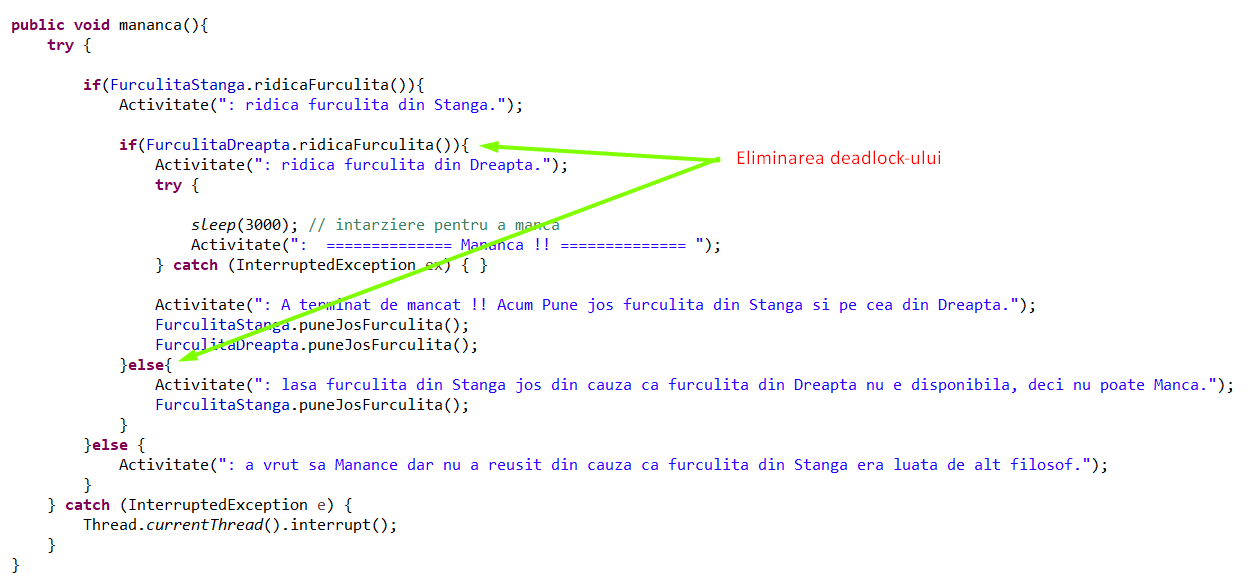
\includegraphics[height=2.8 in, width = 4.9 in]{Eliminare_deadlock.png}
\end{center}

\newpage

\begin{itemize}
\item Implementarea de mai sus are urmatoarele rezultate: 
\end{itemize}

\begin{center}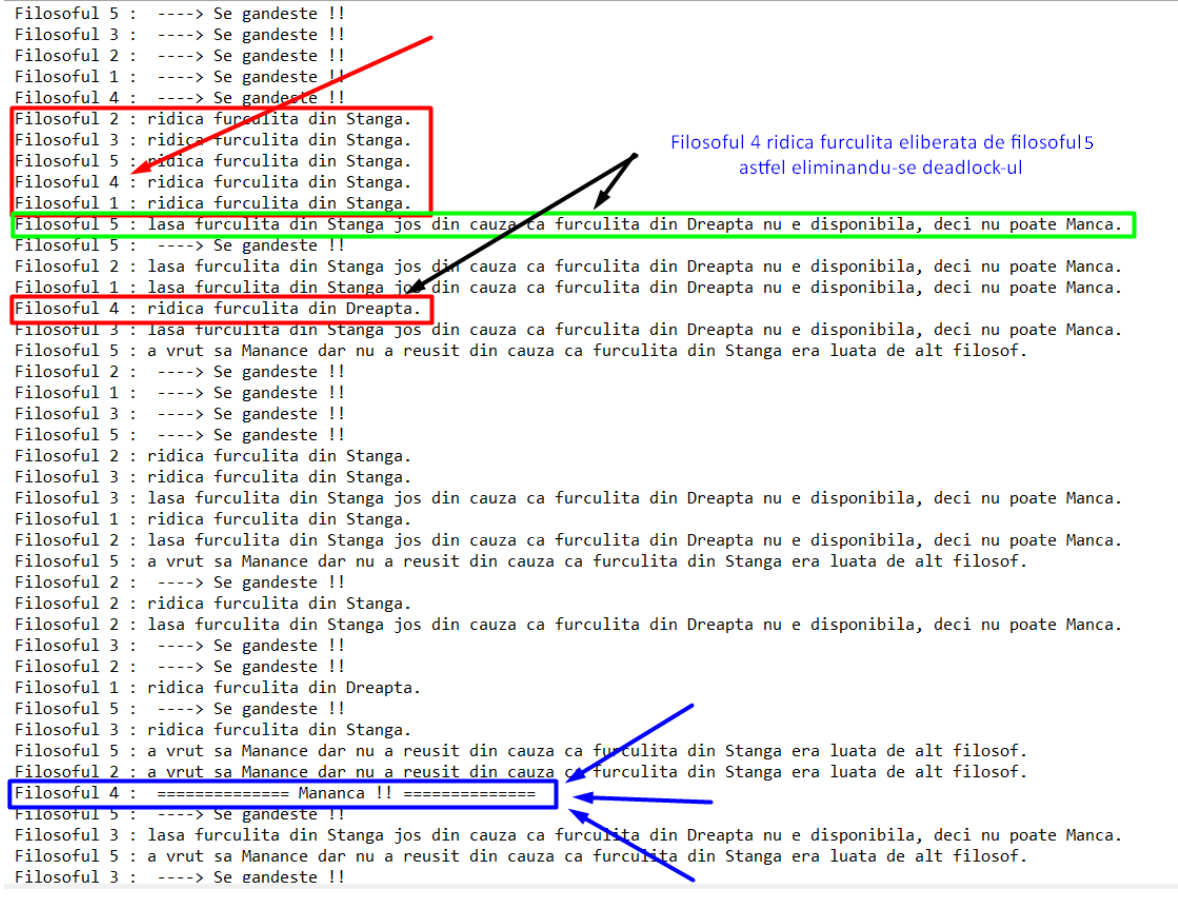
\includegraphics[height=3.9 in, width = 4.9 in]{filosofi_run.png}
\end{center}

\begin{itemize}
\item Mai multe cazuri de test sunt prezentate in directorul "\textit{Date experimentale P2}".
\end{itemize}


\subsection{\textbf{Concluzii}}

\begin{itemize}
\item Implementand aceasta problema mi-am fixat mai bine cunostintele legate de programarea concurenta, am invatat lucruri noi despre comportamentul firelor de executie cat si despre restrictiile ce ar putea fi aplicate asupra firelor astfel incat rezultatul sa fie cel dorit.

\item Utilizarea mecanismelor de sincronizare este extrem de importanta in programarea concurenta. Studiind aceste mecanisme mi-am imbunatatit abilitatile de programare concurenta.


\item Consider ca aceste tipuri de exercitii au fost foarte bine alese pentru partea aceasta de studiu a mecanismelor de sincronizare ale firelor de executie deoarece implementand solutiile unor  cerinte de acest tip ajungi sa intelegi cu adevarat riscurile executiei unui program pe mai multe fire, stii la ce sa te astepti si cum ai putea rezolva anumite "conflicte" dintre firele de executie.

\end{itemize}

\end{document}
